\documentclass{article}
\setlength{\parindent}{2em} % Set the paragraph indent to 2em
\usepackage{graphicx}
\usepackage{hyperref}
\usepackage{tikz}
\usepackage{pgfplots}
\usepackage{multirow} % Make sure this line is present
\usepackage[a4paper, margin=0.5in]{geometry} % Set margins (1 inch in this example)


\author{Croitor Vladimir-Alexandru, Luca Andrei}
\title{Homework 0}

\begin{document}
\maketitle

\section{Introduction}
In this document, we will present the implementation and evaluation of the Iterative Hill Climbing algorithm for optimization tasks. We will discuss the algorithm's structure, including candidate solution representation and neighborhood generation. Additionally, we will compare two improvement methods: the First Improvement Method and the Best Improvement Method, examining their effectiveness in finding optimal solutions.

The algorithm's performance is evaluated using the Rastrigin, Michalewicz, Sphere, and Sum of Squares functions in both 2D and 10D spaces. We will leverage the increase in dimensionality to further highlight the differences between the two improvement algorithms and assess their impact on the overall computational time required for output.

\section{Method}

\subsection{Implementation}


The Iterative Hill Climbing algorithm was implemented using C++. This choice facilitates faster execution, which is crucial for handling computationally intensive optimization tasks. Candidate solutions are represented as boolean vectors, simplifying the process of generating their neighborhoods.For the sake of script reusability, function parameters are organized into separate structs, which are later initialized for their corresponding functions.

To decrease the total wait time for each execution of the algorithm, we employed multithreading. By distributing the workload across multiple threads, we enhance the algorithm's efficiency and improve overall computational speed, resulting in faster outcomes and better resource utilization.
	


\subsection{Neighborhood Generation}
In the Iterative Hill Climbing Algorithm, neighborhoods are created by changing exactly one bit of the candidate solution. This small change produces nearby solutions that are similar to the original one, allowing the algorithm to explore the solution space effectively. By evaluating these neighboring solutions, the algorithm can find better options and improve the overall result. This method keeps the process efficient while helping the algorithm move closer to optimal solutions.



\subsection{Candidate Evaluation}
To evaluate the candidates generated by our algorithm, we begin by converting their representations from binary to decimal form. This process involves segmenting the input bitstring into chunks that correspond to the number of dimensions of our optimization function. Each binary chunk is carefully transformed into its decimal equivalent, ensuring that we accurately capture the intended values. These converted decimal values are then stored in a vector, which organizes the parameters that will be passed to our evaluation function. This allows for a comprehensive assessment of each candidate’s performance using well-known optimization benchmarks within the context of the task.


\subsection{Improvement Methods}
Depending on the value of the boolean parameter passed to the function, our improvement strategy can utilize one of two methods to evaluate an array of neighbors against the initial candidate:

\begin{itemize} 
	\item The First Improvement Method 
	\item The Best Improvement Method 
\end{itemize}

Only one of these methods can be employed for an execution of a script at once.
 
The First Improvement Method compares the initial candidate with each neighbor in its neighborhood vector until it finds a neighbor with a better evaluation than the candidate itself.

In contrast, the Best Improvement Method evaluates all neighbors within the vector to identify the one with the highest evaluation, which is then compared to the initial candidate's evaluation.

If the selected method identifies a better candidate within the neighborhood, this candidate becomes the new initial candidate, prompting the reevaluation of the neighborhood and improvement functions, effectively restarting the process. If the method does not find a better solution than the initial candidate, we conclude that a local minimum of the optimization function has been reached. In this case, we terminate the local loop and begin anew with a different randomly generated candidate.

\section{Experiment}
The algorithm was tested using the Rastrigin, Michalewicz, Sphere, and Sum of Squares functions, with each function evaluated in both its 2D and 10D spaces. The algorithm assessed improvements between candidates with a precision of five decimal places and was run for 10,000 iterations. To ensure the reliability of the results, each experimental run was conducted 30 times to account for variability and minimize the influence of chance.

\section{Results}

\subsection{Rastrigin}

{\Large % Use Huge font size
\[
f(x) = 10 \cdot n + \sum_{i=1}^{n} \left( x_i^2 -10 \cdot \cos(2\pi x_i) \right)
\]

\begin{figure}[h]
    \centering
    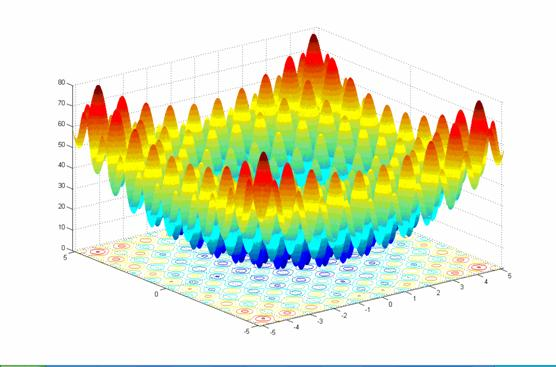
\includegraphics[width=0.8\textwidth]{rastringin.jpg} 
    \caption{Function graph for n=2 \cite{Rastrigin}}
    \label{fig:rastrigin-image}
\end{figure}

}
\begin{table}[ht]
\resizebox{\textwidth}{!}{
\begin{tabular}{|llll|lll|llll|}
\cline{1-4} \cline{8-11}
\multicolumn{4}{|c|}{Best Improvement Results}                                                            &  &  &  & \multicolumn{4}{c|}{First Improvement Results}                                                            \\ \cline{1-4} \cline{8-11} 
\multicolumn{1}{|l|}{Dimension} & \multicolumn{1}{l|}{Best}     & \multicolumn{1}{l|}{Average}  & Worst   &  &  &  & \multicolumn{1}{l|}{Dimension} & \multicolumn{1}{l|}{Best}     & \multicolumn{1}{l|}{Average}  & Worst    \\ \cline{1-4} \cline{8-11} 
\multicolumn{1}{|l|}{D2}        & \multicolumn{1}{l|}{0.00000}  & \multicolumn{1}{l|}{0.00000}  & 0.00000 &  &  &  & \multicolumn{1}{l|}{D2}        & \multicolumn{1}{l|}{0.00000}  & \multicolumn{1}{l|}{0.00000}  & 0.00000  \\ \cline{1-4} \cline{8-11} 
\multicolumn{1}{|l|}{D10}       & \multicolumn{1}{l|}{1.00001} & \multicolumn{1}{l|}{2.31922} & 3.4666  &  &  &  & \multicolumn{1}{l|}{D10}       & \multicolumn{1}{l|}{1.98992} & \multicolumn{1}{l|}{3.94618} & 4.99499 \\ \cline{1-4} \cline{8-11} 
\multicolumn{4}{|c|}{Best Improvement Time}                                                               &  &  &  & \multicolumn{4}{c|}{First Improvement Time}                                                               \\ \cline{1-4} \cline{8-11} 
\multicolumn{1}{|l|}{Dimension} & \multicolumn{1}{l|}{Best}     & \multicolumn{1}{l|}{Average}  & Worst   &  &  &  & \multicolumn{1}{l|}{Dimension} & \multicolumn{1}{l|}{Best}     & \multicolumn{1}{l|}{Average}  & Worst    \\ \cline{1-4} \cline{8-11} 
\multicolumn{1}{|l|}{D2}        & \multicolumn{1}{l|}{6.66783}  & \multicolumn{1}{l|}{6.76448}  &  7.05518 &  &  &  & \multicolumn{1}{l|}{D2}        & \multicolumn{1}{l|}{5.09264}   & \multicolumn{1}{l|}{5.13681}  & 5.27866  \\ \cline{1-4} \cline{8-11} 
\multicolumn{1}{|l|}{D10}       & \multicolumn{1}{l|}{472.293}  & \multicolumn{1}{l|}{476.244}  & 492.402 &  &  &  & \multicolumn{1}{l|}{D10}       & \multicolumn{1}{l|}{318.891}  & \multicolumn{1}{l|}{337.722}  & 353.357  \\ \cline{1-4} \cline{8-11} 
\end{tabular}
}
\end{table}

\clearpage
\subsection{Michalewicz}

{\Large % Use Huge font size
\[
f(x) = -\sum_{i=1}^{n} \sin(x_i) \cdot \left( \sin\left(\frac{i \cdot x_i^2}{\pi}\right) \right)^{20}
\]

\begin{figure}[h]
    \centering
    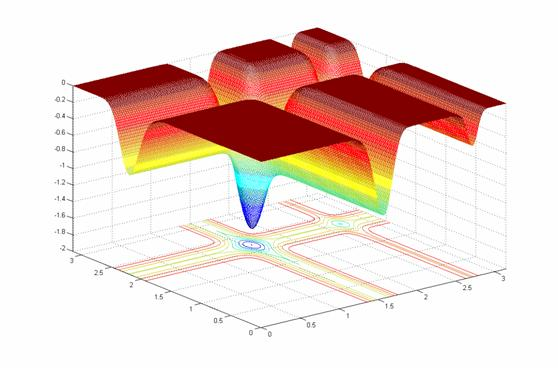
\includegraphics[width=0.8\textwidth]{michalewicz.jpg} 
    \caption{Function graph for n=2 \cite{Michalewicz}}
    \label{fig:rastrigin-image}
\end{figure}

}

\begin{table}[ht]
\resizebox{\textwidth}{!}{
\begin{tabular}{|llll|lll|llll|}
\cline{1-4} \cline{8-11}
\multicolumn{4}{|c|}{Best Improvement Results}                                                            &  &  &  & \multicolumn{4}{c|}{First Improvement Results}                                                            \\ \cline{1-4} \cline{8-11} 
\multicolumn{1}{|l|}{Dimension} & \multicolumn{1}{l|}{Best}     & \multicolumn{1}{l|}{Average}  & Worst   &  &  &  & \multicolumn{1}{l|}{Dimension} & \multicolumn{1}{l|}{Best}     & \multicolumn{1}{l|}{Average}  & Worst    \\ \cline{1-4} \cline{8-11} 
\multicolumn{1}{|l|}{D2}        & \multicolumn{1}{l|}{-1.8013}  & \multicolumn{1}{l|}{-1.8013}  & -1.8013 &  &  &  & \multicolumn{1}{l|}{D2}        & \multicolumn{1}{l|}{-1.8013}  & \multicolumn{1}{l|}{-1.8013}  & -1.8013  \\ \cline{1-4} \cline{8-11} 
\multicolumn{1}{|l|}{D10}       & \multicolumn{1}{l|}{-9.65419} & \multicolumn{1}{l|}{-9.54496} & -9.406  &  &  &  & \multicolumn{1}{l|}{D10}       & \multicolumn{1}{l|}{-9.52621} & \multicolumn{1}{l|}{-9.43526} & -9.31173 \\ \cline{1-4} \cline{8-11} 
\multicolumn{4}{|c|}{Best Improvement Time}                                                               &  &  &  & \multicolumn{4}{c|}{First Improvement Time}                                                               \\ \cline{1-4} \cline{8-11} 
\multicolumn{1}{|l|}{Dimension} & \multicolumn{1}{l|}{Best}     & \multicolumn{1}{l|}{Average}  & Worst   &  &  &  & \multicolumn{1}{l|}{Dimension} & \multicolumn{1}{l|}{Best}     & \multicolumn{1}{l|}{Average}  & Worst    \\ \cline{1-4} \cline{8-11} 
\multicolumn{1}{|l|}{D2}        & \multicolumn{1}{l|}{6.60425}  & \multicolumn{1}{l|}{6.66988}  & 6.77391 &  &  &  & \multicolumn{1}{l|}{D2}        & \multicolumn{1}{l|}{4.6646}   & \multicolumn{1}{l|}{4.71813}  & 4.78248  \\ \cline{1-4} \cline{8-11} 
\multicolumn{1}{|l|}{D10}       & \multicolumn{1}{l|}{416.104}  & \multicolumn{1}{l|}{424.096}  & 441.359 &  &  &  & \multicolumn{1}{l|}{D10}       & \multicolumn{1}{l|}{269.221}  & \multicolumn{1}{l|}{275.021}  & 286.482  \\ \cline{1-4} \cline{8-11} 
\end{tabular}
}
\end{table}
\clearpage
\subsection{Sphere}

{\Large % Use Huge font size
\[
f(x) = \sum_{i=1}^{n} x_i^2                         
\]

\begin{figure}[h!]
    \centering
    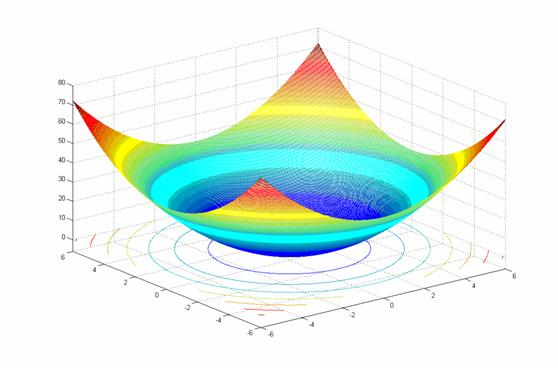
\includegraphics[width=0.8\textwidth]{sphere.jpg} 
    \caption{Function graph for n=2 \cite{Sphere}}
    \label{fig:rastrigin-image}
\end{figure}

}
\begin{table}[ht]
\resizebox{\textwidth}{!}{
\begin{tabular}{|llll|lll|llll|}
\cline{1-4} \cline{8-11}
\multicolumn{4}{|c|}{Best Improvement Results}                                                            &  &  &  & \multicolumn{4}{c|}{First Improvement Results}                                                            \\ \cline{1-4} \cline{8-11} 
\multicolumn{1}{|l|}{Dimension} & \multicolumn{1}{l|}{Best}     & \multicolumn{1}{l|}{Average}  & Worst   &  &  &  & \multicolumn{1}{l|}{Dimension} & \multicolumn{1}{l|}{Best}     & \multicolumn{1}{l|}{Average}  & Worst    \\ \cline{1-4} \cline{8-11} 
\multicolumn{1}{|l|}{D2}        & \multicolumn{1}{l|}{0.00000}  & \multicolumn{1}{l|}{0.00000}  & 0.00000 &  &  &  & \multicolumn{1}{l|}{D2}        & \multicolumn{1}{l|}{0.00000}  & \multicolumn{1}{l|}{0.00000}  & 0.00000  \\ \cline{1-4} \cline{8-11} 
\multicolumn{1}{|l|}{D10}       & \multicolumn{1}{l|}{0.00000} & \multicolumn{1}{l|}{0.00000} & 0.00000  &  &  &  & \multicolumn{1}{l|}{D10}       & \multicolumn{1}{l|}{0.00000} & \multicolumn{1}{l|}{0.00000} & 0.00000 \\ \cline{1-4} \cline{8-11} 
\multicolumn{4}{|c|}{Best Improvement Time}                                                               &  &  &  & \multicolumn{4}{c|}{First Improvement Time}                                                               \\ \cline{1-4} \cline{8-11} 
\multicolumn{1}{|l|}{Dimension} & \multicolumn{1}{l|}{Best}     & \multicolumn{1}{l|}{Average}  & Worst   &  &  &  & \multicolumn{1}{l|}{Dimension} & \multicolumn{1}{l|}{Best}     & \multicolumn{1}{l|}{Average}  & Worst    \\ \cline{1-4} \cline{8-11} 
\multicolumn{1}{|l|}{D2}        & \multicolumn{1}{l|}{8.37554}  & \multicolumn{1}{l|}{8.45058}  & 8.56522 &  &  &  & \multicolumn{1}{l|}{D2}        & \multicolumn{1}{l|}{4.6646}   & \multicolumn{1}{l|}{4.71813}  & 4.78248  \\ \cline{1-4} \cline{8-11} 
\multicolumn{1}{|l|}{D10}       & \multicolumn{1}{l|}{416.104}  & \multicolumn{1}{l|}{424.096}  & 441.359 &  &  &  & \multicolumn{1}{l|}{D10}       & \multicolumn{1}{l|}{269.221}  & \multicolumn{1}{l|}{275.021}  & 286.482  \\ \cline{1-4} \cline{8-11} 
\end{tabular}
}
\end{table}


\clearpage
\subsection{Sum Square}

{\Large % Use Huge font size
\[
f(x) = \sum_{i=1}^{n} i \cdot x_i^2                 
\]

\begin{figure}[h!]
    \centering
    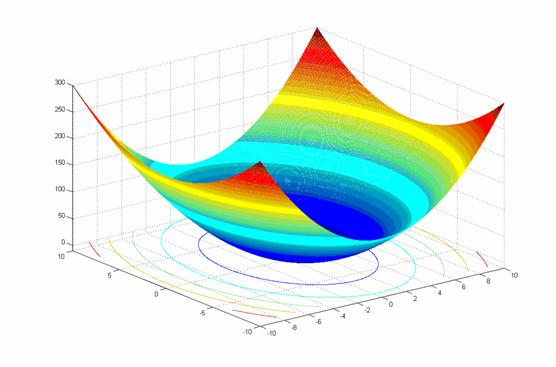
\includegraphics[width=0.8\textwidth]{sum_square.jpg} 
    \caption{Function graph for n=2 \cite{Sum_Square}}
    \label{fig:rastrigin-image}
\end{figure}

}
\begin{table}[]
\resizebox{\textwidth}{!}{
\begin{tabular}{|llll|lll|llll|}
\cline{1-4} \cline{8-11}
\multicolumn{4}{|c|}{Best Improvement Results}                                                     &  &  &  & \multicolumn{4}{c|}{First Improvement Results}                                                     \\ \cline{1-4} \cline{8-11} 
\multicolumn{1}{|l|}{Dimension} & \multicolumn{1}{l|}{Best} & \multicolumn{1}{l|}{Average} & Worst &  &  &  & \multicolumn{1}{l|}{Dimension} & \multicolumn{1}{l|}{Best} & \multicolumn{1}{l|}{Average} & Worst \\ \cline{1-4} \cline{8-11} 
\multicolumn{1}{|l|}{D2}        & \multicolumn{1}{l|}{}     & \multicolumn{1}{l|}{}        &       &  &  &  & \multicolumn{1}{l|}{D2}        & \multicolumn{1}{l|}{}     & \multicolumn{1}{l|}{}        &       \\ \cline{1-4} \cline{8-11} 
\multicolumn{1}{|l|}{D10}       & \multicolumn{1}{l|}{}     & \multicolumn{1}{l|}{}        &       &  &  &  & \multicolumn{1}{l|}{D10}       & \multicolumn{1}{l|}{}     & \multicolumn{1}{l|}{}        &       \\ \cline{1-4} \cline{8-11} 
\multicolumn{4}{|c|}{Best Improvement Time}                                                     &  &  &  & \multicolumn{4}{c|}{First Improvement Time}                                                     \\ \cline{1-4} \cline{8-11} 
\multicolumn{1}{|l|}{Dimension} & \multicolumn{1}{l|}{Best} & \multicolumn{1}{l|}{Average} & Worst &  &  &  & \multicolumn{1}{l|}{Dimension} & \multicolumn{1}{l|}{Best} & \multicolumn{1}{l|}{Average} & Worst \\ \cline{1-4} \cline{8-11} 
\multicolumn{1}{|l|}{D2}        & \multicolumn{1}{l|}{}     & \multicolumn{1}{l|}{}        &       &  &  &  & \multicolumn{1}{l|}{D2}        & \multicolumn{1}{l|}{}     & \multicolumn{1}{l|}{}        &       \\ \cline{1-4} \cline{8-11} 
\multicolumn{1}{|l|}{D10}       & \multicolumn{1}{l|}{}     & \multicolumn{1}{l|}{}        &       &  &  &  & \multicolumn{1}{l|}{D10}       & \multicolumn{1}{l|}{}     & \multicolumn{1}{l|}{}        &       \\ \cline{1-4} \cline{8-11} 
\end{tabular}
}
\end{table}


\section{Conclusions}
The results of the experiments highlight the key differences between the Best Candidate Method and the First Candidate Method. While the First Candidate Method produces results in a relatively short amount of time, it may sacrifice optimality to achieve this performance; nonetheless, its results remain fairly accurate. In contrast, the Best Candidate Method prioritizes accuracy over time efficiency.

Furthermore, there is a significant increase in required time between the 2D and 10D versions of the same function, underscoring the impact of the number of parameters on the average convergence time of the algorithm.


\clearpage
\begin{thebibliography}{9}

\bibitem{Rastrigin}
  Rastrigin's Function rendered image. \\
  \url{http://www-optima.amp.i.kyoto-u.ac.jp/member/student/hedar/Hedar_files/TestGO_files/Page2607.htm}

\bibitem{Michalewicz}
  Michalewicz's Function rendered image. \\
  \url{http://www-optima.amp.i.kyoto-u.ac.jp/member/student/hedar/Hedar_files/TestGO_files/Page2376.htm}

  \bibitem{Sphere}
  Sphere Function rendered image. \\
  \url{http://www-optima.amp.i.kyoto-u.ac.jp/member/student/hedar/Hedar_files/TestGO_files/Page1113.htm}

  \bibitem{Sum_Square}
  Sum Square Function rendered image. \\
  \url{http://www-optima.amp.i.kyoto-u.ac.jp/member/student/hedar/Hedar_files/TestGO_files/Page674.htm}

\end{thebibliography}  
\end{document}
